
\newcommand{\gr}[1]{\textcolor{red}{#1}}
\newcommand{\lh}[1]{\textcolor{purple}{#1}}
\newcommand{\kl}[1]{\textcolor{blue}{#1}}
\documentclass[5p,times,a4paper,fleqn]{cas-dc}
\usepackage{xeCJK}
\usepackage{amsmath}

\usepackage[numbers]{natbib}
\usepackage{todonotes}
\usepackage[linesnumbered,ruled,vlined]{algorithm2e}
\usepackage{ulem}
\usepackage{multirow}
\usepackage{float}
\restylefloat{table}
\def\tsc#1{\csdef{#1}{\textsc{\lowercase{#1}}\xspace}}
\tsc{WGM}
\tsc{QE}
\tsc{EP}
\tsc{PMS}
\tsc{BEC}
\tsc{DE}
\begin{document}
   \let       \WriteBookmarks       \relax    
   \def       \floatpagepagefraction{1}    
   \def       \textpagefraction{.001}    
   \shorttitle{Extending DD-        $\alpha$        AMG on heterogeneous machines}    
   \shortauthors{He, Ramirez-Hidalgo, Zhang}    
   \title[mode = title]{在异构机器上扩展 DD-  $\alpha$  AMG  }     

   \author[1]{Lianhua He}    []
   \fnmark    [1]
   \ead{helh@sccas.cn}    
   \affiliation[1]{organization={Computer Network Information Center, Chinese Academy of Sciences},
    addressline={CAS Informatization Plaza No.2 Dong Sheng Nan Lu, Haidian District},
    city={Beijing},
    country={China}}    
   \author[2]{Gustavo Ramirez-Hidalgo}    []
   \fnmark    [2]
   \ead{g.ramirez@math.uni-wuppertal.de}    
   \affiliation[2]{organization={Department of Mathematics, Bergische Universität Wuppertal},
    addressline={Gaußstraße 20},
    city={Wuppertal},
    postcode={42097}, 
    country={Germany}}    
   \author[1]{Ke-Long Zhang}    
   \cormark    [1]
   \fnmark    [1]
   \ead{klzhang@cnic.cn}     

   \begin{abstract}多重网格求解器是现代科学计算模拟的标准。基于域分解聚合的代数多重网格,也称为 DD-   $\alpha$    AMG 求解器,是格子量子色动力学代数多重网格求解器的成功实现。它的 CPU 实现使得为某些特定的离散化构建计算上不可行模拟成为可能,此外,它还推动了该领域其他代数多重网格求解器的开发和改进。从现有版本的 DD-   $\alpha$    AMG 开始,该版本已通过    \texttt{CUDA}    部分移植,以在 Nvidia GPU 上运行多重网格求解器的一些最精细级别的操作,我们在此处使用    \texttt{HIP}    转换    \texttt{CUDA}    代码以在 ORISE 超级计算机上运行。此外,我们还扩展了 DD-   $\alpha$    AMG 中可用的平滑器,特别关注 Richardson 平滑,在我们的数值实验中,这使得多重网格求解器比使用 GCR 的平滑器更快,与 SAP 平滑器相比仅慢 10 \%。然后,我们通过    \texttt{CUDA}    移植了奇偶预处理版本的 GMRES 和 Richardson。最后,我们通过高级矢量化扩展了一些计算密集型粗网格操作。  \end{abstract}    
   \begin{keywords}
GPU \sep multigrid \sep lattice QCD \sep smoother \sep AVX
\end{keywords}     

   \maketitle     

   \section{介绍  }     

强力是自然界四种基本力之一,它由量子色动力学 (QCD) 理论 (QMATHX\_3 ) 建模。由于模型本身的原因,QCD 在某些能量范围内无法进行分析求解,为了在这种情况下获得预测,必须通过所谓的格子 QCD (LQCD)    \cite{gattringer2009quantum}    采用数值方法。就高性能计算 (HPC) 使用而言,LQCD 模拟是科学计算中最苛刻的应用之一。此外,LQCD 模拟中最常见和最昂贵的“基本”操作之一是求解形式为    $Dx = b$    的线性系统,其中    $D$    是狄拉克算子。    $D$    的形式因离散化过程而异,从而产生不同的 LQCD 公式,例如威尔逊、扭曲质量、交错和其他    \cite{gattringer2009quantum,wilson1974confinement,frezzotti2000local,kogut1975hamiltonian}    。  

多重网格方法是解决 LQCD 中线性系统问题的最新方法。具体来说,使用代数多重网格 (AMG) 方法    \cite{trottenberg2000multigrid}    而不是几何方法是解决此问题的必要条件。LQCD 中 AMG 求解器的当前状态源自 20 年的算法和计算持续发展    \cite{Babich2010,Brannick2008,
Brower2020,Frommer2014,osborn2010multigrid}    。  

在 LQCD 环境中,AMG 求解器的一个实现是 DD-    $\alpha$    AMG    \cite{rottmann2016adaptive,Frommer2014}    。该求解器最初在    \texttt{C}    中开发为纯 CPU 代码,通过    \texttt{MPI}    和    \texttt{OpenMP}    并行化,并使用    \texttt{SSE}    矢量化,最近,它的一些最昂贵的部分已通过    \texttt{CUDA}    
   \cite{RamirezHidalgo_PhDThesis,arxivAcceleratingLattice}    移植到 GPU 上运行。我们从这个混合 CPU+GPU 版本开始,并使用    \texttt{HIP}    对其进行扩展,使其在 ORISE 超级计算机上运行,然后我们在算法和计算上扩展    \texttt{C}    和    \texttt{CUDA}    代码,最后升级一些粗网格内核以支持    \texttt{AVX2}    和    \texttt{AVX-512}    而不是    \texttt{SSE}    。  

本文内容如下。第    \ref{sect:amg_and_orise}    节通过描述 ORISE 超级计算机 AMG 和 DD-   $\alpha$    AMG 来设定背景,然后描述和比较与本文中完成的 DD-   $\alpha$    AMG 扩展相关的迭代方法,最后我们描述和比较    \texttt{CUDA}    和    \texttt{HIP}   。然后,第    \ref{sect:num_exps}    节介绍数值实验,我们讨论了此处实现的 DD-   $\alpha$    AMG 扩展,并在 ORISE 上运行,最后我们通过讨论通过    \texttt{AVX}    进行的 CPU 改进的影响来结束本节。最后,我们在第    \ref{sect:conclusions_and_future_work}    节中提出结论以及当前和未来的工作。  

   \section{通过    \texttt{HIP}    在 ORISE 上进行多重网格  }       \label{sect:amg_and_orise}     

在本工作中,我们除其他工作外,还通过异构计算可移植接口 (   \texttt{HIP}   )    \cite{HIPdocum88:online,HIP_GitHub}    翻译了当前的 CPU+GPU 版本的 DD-   $\alpha$    AMG    \cite{wuppertalGPUDDalphaAMG}   。第    \ref{subsect:smoothers_comp_cpu_only}    和    \ref{subsect:ddalphaamg_on_orise_results}    小节中介绍的数值实验在 ORISE 超级计算机上运行,因此我们从描述 ORISE 中的架构开始本节。接下来是 AMG 和 AMG 求解器 DD-   $\alpha$    AMG 的简要介绍,后者将在此处进行扩展。然后,我们对 DD-   $\alpha$    AMG 中用作平滑器的两种迭代方法进行了比较描述:广义最小残差 (GMRES) 方法和 Schwarz 交替生成 (SAP),特别讨论了它们在平滑和在 CPU 和 GPU 上运行方面的优缺点;我们通过在平滑器堆栈中添加两种迭代方法(广义共轭残差 (GCR) 和改进的 Richardson)来扩展讨论(以及 DD-   $\alpha$    AMG 本身)。我们通过简要描述    \texttt{CUDA}    和    \texttt{HIP}    来结束本节,强调它们的差异和相似之处。  

   \subsection{ORISE超级计算机  }     

该机器由配备 GPU 的 CPU 节点组成。在 CPU 方面,每个节点都是 4 路 8 核,总共 32 个核心,具有 x86 指令集和 128 GB RAM。它支持 POSIX 标准和 MPI、OpenMP 等常见的并行编程模型。每个节点都连接了四个 GPU。单个 GPU 由 64 个流式多处理器和 16 GB HBM2 RAM 组成。每个节点通过 32 个 PCIe 总线连接到其 GPU 加速器。每个加速器通过带宽为 16 GB/s 的直接内存访问 (DMA) 访问其相应的 CPU,节点通过带宽为 25 GB/s 的高速网络连接。ORISE 能够使用    \texttt{HIP}    在其 GPU 上运行基于    \texttt{CUDA}    的应用程序。  

在 ORISE 中无法进行直接的 GPU 到 GPU 通信,因此我们在实现中采用更昂贵的程序,即先进行 GPU 到 CPU 通信,然后再进行 CPU 到 GPU 通信,以便能够将数据从一个 GPU 传送到另一个 GPU。  

   \subsection{代数多重网格  }       \label{subsect:amg}     

一般在求解线性组    $Dx = b$    时,传统的迭代法如雅可比、高斯-赛德尔、GMRES 等~    \cite{saad2003iterative}    ,虽然在很多方面各不相同,但它们都有一个共同的缺点:随着矩阵    $D$    即 \     $\kappa(D)$    的条件数的增加,它们达到一定相对容差的迭代次数也会增加,有时还会非常快。另一方面,随着科学计算模拟中的参数越来越接近连续参数,一些出现在线性组中待求解矩阵的条件数会迅速增长。  

多重网格法    \cite{trottenberg2000multigrid}    的诞生源于人们希望拥有一个收敛与    $\kappa(D)$    无关的求解器。为了实现这种独立性,平滑器和粗网格相结合。平滑器由传统方法(例如 \  Gauss-Seidel、GMRES)的几次迭代组成。只需几次迭代,此类方法就可以快速消除与    $D$    的大特征值    \footnote{对于本小节的其余部分,我们用    $e_{low}$    表示与    $D$    和    $e_{high}$    的小特征值(幅度)近似相关的部分误差,这些特征值与大特征值相关。  }    相关的误差分量,但它们会在某个时候停滞不前,因为这些算法不易处理与    $D$    的小特征值相对应的误差分量。这时,多重网格法就会变得有益,甚至是必要的。在传统方法的几次迭代之后,使用粗网格,并将与误差相关的信息从细网格传输到粗网格。在粗网格上计算误差的近似值,然后传输回细网格并校正当前的近似值。现在让我们将多重网格描述为一个逐步的过程:
   \begin{enumerate}

    \item   设置    $i \leftarrow 0$    和初始猜测    $x^{(0)}$    。   \item   设置    $i \leftarrow i+1$    。设置    $x^{(i)} \leftarrow x^{(i-1)}$    。更新残差    $r^{(i)} \leftarrow b - D x^{(i)}$    ,检查停止条件并在必要时停止。根据误差和残差    $D e^{(i)} = r^{(i)}$    之间的关系,执行预平滑    $M^{(\nu)}$    的    $\nu$    次迭代,以此获得    $\widehat{e}^{(i)} \leftarrow M^{(\nu)} r^{(i)}$    。然后校正当前迭代,即 \     $x^{(i)} \leftarrow x^{(i)} + \widehat{e}^{(i)}$    。更平滑的    $M^{(\nu)}$    可有效近似抑制    $e_{high}$    ,使新的误差    $e^{(i)}$    在    $D$    的大特征模式中不那么丰富。   \item   更新残差    $r^{(i)} \leftarrow b - D x^{(i)}$    。通过线性变换    $P$    和    $R$    分别将数量传入和传出粗网格,使用    $\widehat{e}^{(i)} \leftarrow P D_{c}^{-1} R r^{(i)}$    和    $D_{c} = R D P$    进行形式为    $x^{(i)} \leftarrow x^{(i)} + \widehat{e}^{(i)}$    的粗网格校正(可有效近似地去除    $e_{low}$    )会导致新的误差    $e^{(i)}$    ,其中许多与    $D$    的小特征模式相关的误差分量被进一步抑制。   \item   更新残差    $r^{(i)} \leftarrow b - D x^{(i)}$    。后平滑的应用方式与预平滑相同,即 \  我们得到    $x^{(i)} \leftarrow x^{(i)} + \widehat{e}^{(i)}$    和    $\widehat{e}^{(i)} \leftarrow M^{(\nu)} r^{(i)}$    。检查停止标准,如果完成则停止,否则转到步骤 2。  \end{enumerate}     

上面列出的两级方法可以进一步以递归方式使用,因为    $D_{c}^{-1} R r^{(i)}$    操作中的矩阵    $D_{c}$    可能太大而无法使用直接方法求逆,或者太病态而无法使用传统方法(例如 \  重新启动 GMRES),因此我们可能希望递归地使用另一个两级方法来求解系统    $D_{c} x_{c} = R r^{(i)}$    ,从而使该方法成为多级方法。  

我们使用的是几何    \cite{briggs2000multigrid,wesseling2001geometric}    还是代数    \cite{stuben2001introduction,falgout2006introduction}    多重网格取决于我们用于构建    $P$    和    $R$    的信息。在几何多重网格中,网格结构是唯一需要的要素,例如 \  可以设计    $P$    ,使其在从粗网格到细网格时在晶格点上插入值(即 \  平均值),然后可以选择例如    $R = P^{H}$    。这种    $R = P^{H}$    的选择称为 Galerkin 构造    \cite{briggs2000multigrid}    。  

在代数多重网格方法中,使用矩阵    $D$    中的数据来构建    $P$    和    $R$    是基本方法。让我们简要详细地介绍一下这一点。假设    $P$    的列跨度近似于    $D$    的许多小特征模所跨越的子空间,即 \     $\texttt{range}(P) \approx \texttt{range}(V)$    ,其中    $V$    的列包含    $D$    的许多最小特征向量。然后,我们可以将某个向量    $u$    写为    $e_{low} \approx Pu$    。粗网格校正,即 \     $x^{(i)} \leftarrow x^{(i)} + P D_{c}^{-1} R r^{(i)}$    ,可以等效地以误差更新的形式写为    $e^{(i)} \leftarrow (I - P D_{c}^{-1} R D) e^{(i)}$    ,进而得到    $e_{low}^{(i)} \leftarrow (I - P D_{c}^{-1} R D) e_{low}^{(i)} \approx Pu - P D_{c}^{-1} R D Pu = 0$    。因此,我们看到,   $\texttt{range}(P)$    富含    $D$    的小特征模式,这为我们提供了良好的粗网格校正。下一小节将讨论 LQCD 的 AMG 求解器的实现。  

   \subsection{基于区域分解聚合的代数多重网格  }       \label{subsect:ddalphaamg}     

基于域分解聚合的代数多重网格 (DD-    $\alpha$    AMG)    \cite{rottmann2016adaptive,Frommer2014}    既是用于解决 LQCD 中线性系统的算法框架,也是代码    \cite{wuppertalDDalphaAMG}   。它针对 Wilson-Dirac 离散化并进行了三叶草改进。  

对于 LQCD 的狄拉克算子,需要从    $D$    代数构造    $P$   。DD-    $\alpha$    AMG 通过基于聚合的 AMG 实现此操作。这种基于聚合的构造依赖于局部相干性    \cite{luscher2007local}    的概念,该概念指出,通过查看这几种模式的局部行为,可以从少数几种低模式近似获得    $D$    的许多低模式。通过这种构造,我们可以将    $D$    的许多近似低模式作为    $P$    的列,其中    $P$    中的稀疏结构导致粗网格狄拉克算子    $D_{c}$    在其最近邻结构中类似于    $D$   。在细网格中,每个格点的自由度 (d.o.f.) 为 12,因此    $D$    每 12 行有 9 个    $12 \times 12$    块,而对于    $D_{c}$   ,此结构相同,只是现在每    $2N_{v}$    行有 9 个    $2N_{v} \times 2N_{v}$    块。数量    $N_{v}$    称为测试向量的数量,它们是我们用于构建    $P$    的近似低模式;典型值为    $N_{v} = 24$    。在多级设置中(即 \  超过两个级别),下一个粗网格通过近似    $D_{c}$    的低模式以递归方式构建。  

DD-    $\alpha$    AMG 求解器具有设置阶段和求解阶段。在设置阶段,它会构建多重网格层次结构。让我们将此多重网格层次结构定义为运算符集    $D_{\ell}$    与    $\ell = 1, ..., L$    以及    $P_{\ell}$    和    $R_{\ell} = P_{\ell}^{H}$    与    $\ell = 1, ..., L-1$    ,   $L$    为总级别数。然后,求解阶段会利用此运算符层次结构求解一个或多个线性系统,即序列中一个或多个右侧的 \ 。  

在求解阶段,DD-    $\alpha$    AMG 在除最粗级以外的每一级都使用由两级 AMG 预处理的灵活 GMRES    \cite{saad2003iterative}    (FGMRES)。细网格上的 FGMRES 求解至所需的相对残差公差,例如 \     $10^{-12}$    。如果使用两级,则通过 GMRES 求解粗网格线性系统,直至相对残差公差为    $10^{-1}$    ;如果使用两级以上,则使用 FGMRES 代替 GMRES,仍然直至    $10^{-1}$    ,但现在由另一种两级方法预处理,从而产生三级求解器。这种循环策略,即 \  使用 FMGRES 来包裹多重网格求解器的每一级,称为 K 循环    \cite{notay2008recursive}    。  

在 DD-    $\alpha$    AMG 中,较粗级别的 (F)GMRES 通常求解至    $10^{-1}$    。对于更平滑的级别,可以选择 GMRES 或 SAP 之一,我们将在小节    \ref{subsect:smoothers_comp}    中进一步讨论这一点。如果多重网格求解器的参数选择得当,随着    $D$    的条件变大,最精细级别的 FGMRES 达到所需容差的迭代次数将基本保持不变。随着    $\kappa(D)$    的增加,会出现更多病态的较粗级别,这尤其会影响最粗级别,即 \ ,随着    $\kappa(D)$    的增加,我们将看到求解器收敛的执行时间增加,主要是由于在最粗级别上达到所需的    $10^{-1}$    的迭代次数增加。可以为最粗糙的级别配备预处理和紧缩功能,以在求解器的总执行时间内部分恢复对    $\kappa(D)$    的不敏感性,如    \cite{espinoza2023coarsest}    中所述。  

   \subsection{平滑剂  }       \label{subsect:smoothers_comp}     

在 DD-    $\alpha$    AMG    \cite{wuppertalDDalphaAMG}    的原始版本(仅限 CPU 的代码)中,提供了两个平滑器:GMRES 和 SAP。在较新的 CPU+GPU 版本    \cite{wuppertalGPUDDalphaAMG}    中,最精细级别的 SAP 通过    \texttt{CUDA}    移植到 GPU 上运行,而其余代码则继续在 CPU 上执行。在这项工作中,我们扩展了 CPU 版本以支持 GCR 和修改后的 Richardson 作为平滑器。此外,我们还实现了    \texttt{CUDA}    代码,以便求解器现在能够在 SAP、GMRES 或 Richardson 卸载到 GPU 的情况下运行。  

第 1 节介绍了比较不同平滑器的数值测试。现在,我们将描述、讨论和比较这些测试中考虑的四种平滑器。如果我们讨论奇偶预处理(我们将在第 2 节中进行讨论),就可以更好地理解这四种迭代方法在实际设置中如何充当平滑器,以及它们在 DD-   $\alpha$    AMG 中是如何实际实现的。  

   \subsubsection{树液  }     

SAP 的伪代码在算法~    \ref{alg:sap}    中给出。我们现在解释如何在 DD-    $
\alpha$    AMG 中实现 SAP。对格进行域分解,将其划分为由格的四维块组成的连续但不相交的区域;此域分解可以与过程分解相匹配,但在 DD-    $\alpha$    AMG 中,出于算法和计算性能考虑,在定义 SAP 使用的域分解时使用过程分解的细化。将格分解为块后,对块进行编号和着色(两种颜色,例如红色和黑色),以使没有两个连续的块共享相同的颜色。最后,算法~    \ref{alg:sap}    首先运行红色块,近似求解每个块上定义的线性系统,然后处理黑色块,并将这两个步骤用 for 循环包装起来。块求解是通过最小残差    \cite{saad2003iterative}    完成的,我们写入 SAP(   $n$   ,    $m$   ) 来指示 Schwarz 平滑器中的    $n$    外迭代,其中用于求解块线性系统的最小残差的    $m$    迭代。  

为了更平稳、更快速地移除与    $D$    的大特征模式相关的误差分量,SAP 中的局部更新与要抑制的这种“高频”误差产生更大的共鸣。另一方面,从计算性能的角度来看,全局点积往往会带来问题,因为它们会损害强扩展性,而 SAP 可以缓解这一问题,因为 SAP(   $n$   、   $m$   )中的点积仅具有局部性质。此外,如果域分解块足够小,则一次在一个本地 SAP 块上运行最小残差可能会导致大量缓存重用。  

   \begin{algorithm}
\caption{SAP(   $n$   ,   $m$   )  } \label{alg:sap}
\KwIn{initial guess         $x^{(0)}$        , matrix         $D$        , right hand side         $b$        , SAP iterations         $n$        , number of domain-decomposition blocks         $n_b$        , Minimal Residual iterations         $m$        }
\KwOut{        $x^{(n)}$        }
\For{         $i=1,...,n$        }{
          $x^{(i)} = x^{(i-1)}$        ,         $r^{(i)}=b-Dx^{(i)}$         \\ 
  check convergence via         $\|r^{(i)}\|_{2}$         and exit if done \\ 
  \For{        $k=1,...,n_b$        }{
    \If{color[k]==red}{
      perform Minimal Residual to solve         $D e^{(i)}_k=r^{(i)}_k$         on a single block         $k$        , then         $x_{k}^{(i)}=x_{k}^{(i)}+e_{k}^{(i)}$        
      }
    }
            $r^{(i)}=b-Dx^{(i)}$         \\ 
  \For{        $k=1,...,n_b$        }{
    \If{color[k]==black}{
      perform Minimal Residual to solve         $D e^{(i)}_k=r^{(i)}_k$         on a single block         $k$        , then         $x^{(i)}_k=x^{(i)}_k+e^{(i)}_k$        
      }
    }
}
\end{algorithm}     

   \subsubsection{通用剩余容量  }     

GMRES    \cite{saad1986}    是一种著名且常用的非 Hermitian 系统求解器。通过 Arnoldi 过程,GMRES 构建一个 Krylov 子空间    $\mathcal{K}_{m}(D,r^{(0)})$   ,从中提取信息,通过残差最小化过程近似    $D e^{(0)} = r^{(0)}$    中的误差。对于矩阵    $D \in \mathbb{C}^{d \times d}$    ,GMRES 最多在    $d$    次迭代中收敛,但实际上它在    $n \ll d$    中收敛。在大规模科学计算模拟中,   $n$    的值通常过大,因此改用重新启动的 GMRES(    $n$    ,    $m$    ),我们在 alg.~    \ref{alg:gmres}    中概述了这一点。即使重新启动,GMRES 在求解线性系统时也可能过于昂贵;在这种情况下,可以求助于预处理    \cite{saad2003iterative}   。  

与 SAP 相比,GMRES 的一个缺点是需要全局点积,因此使用后者时强扩展性更好。此外,GMRES 中 Dirac 算子的频繁全局应用(参见算法 \     \ref{alg:gmres}    中的第 5 行)与其中第 2、7 和 8 行中的全局点积相结合,当局部格(即 \  每个    \texttt{MPI}    进程的格大小)很大时,很难实现缓存友好的执行。另一方面,GMRES 可以更快地在整个格中传输更新的数据,这在系统不是太病态并且多重网格求解器更依赖于平滑器的全局收敛时非常方便。  

   \begin{algorithm}
\caption{GMRES(   $n$   ,   $m$   )  } \label{alg:gmres}
\KwIn{initial guess         $x^{(0)}$        , matrix         $D$        , right hand side         $b$        , number of cycles         $n$        , cycle length         $m$        }
\KwOut{        $x^{(n)}$        }
\For{         $i = 1,{\ldots},n$        }{
          $x^{(i)} = x^{(i-1)}$        ,         $r^{(i)} = b - Dx^{(i)}$        ,         $ \beta=h_{1,0}=\left\| r^{(i)} \right\|_2$          \\ 
  check convergence via         $\beta$         and exit if done \\ 
  \For{         $k=1,...,m$        }{
               $v_k = r^{(i)}/h_{k,k-1}$        ,         $w = D v_k$         \\ 
        \For{        $j=1,$        ...        $,k$        }{
                    $h_{j, k}=\left(w,v_j\right) $        ,         $ w=w-h_{j, k} v_j$        
        }
                $h_{k+1, k}=\left\|w\right\|_2$          
  }
  define         $V_k=\left[v_1, \cdots, v_k\right], H_k=\left \{ h_{i, j}\right \} _{1 \leq i \leq k+1,1 \leq j \leq k}$         \\ 
  compute         $y_k=\arg \min _y\left\|\beta e_1-H_k y_k\right\|_2$         and update the current iterate         $x^{(i)} = x^{(i)}+V_k y_k$          \\ 
}
\end{algorithm}     

   \subsubsection{气相色谱  }       \label{subsubsect:gcr}     

GCR    \cite{elman1982iterative}    是一种同样适用于非厄米系统的 Krylov 方法,它在数学上等同于 GMRES,同样最小化了仿射空间    $x^{(0)} + \mathcal{K}_{m}(D,r^{(0)})$    中的残差。不使用正交基,而是将 Krylov 子空间中的向量    $p_{k}$    设为    $D^{H}D$    正交,这是 GCR 中通过将下一个向量(即 \     $p_{k+1}$   )作为当前残差和前一个 Krylov 向量    $p_{i},  \  i \leq k$    的线性组合来进一步约束这一一般条件。算法 \     \ref{alg:gcr}    显示了 GCR 的一种可能公式,它将矩阵    $D$    的应用次数限制为每次迭代一次。  

   \begin{algorithm}
\caption{GCR(   $n,m$   )  } \label{alg:gcr}
\KwIn{initial guess         $x^{(0)}$        , matrix         $D$        , right hand side         $b$        , number of cycles         $n$        , cycle length         $m$        }
\KwOut{        $x^{(n)}$        }
\For{         $i = 1,{\ldots},n$        }{
           $x^{(i)} = x^{(i-1)}$        ,         $r^{(i)} = b - Dx^{(i)}$          \\ 
   check convergence via         $\|r^{(i)}\|_{2}$         and exit if done \\ 
           $p_{1} = r^{(i)}$        ,         $z_{1} = D p_{1}$          \\ 
   \For{         $k=1,...,m$        }{
             $\delta_{k} = (z_{k},z_{k})$          \\ 
             $\alpha = \frac{(r^{(i)},z_{k})}{\delta_{k}}$          \\ 
             $x^{(i)} = x^{(i)} + \alpha p_{k}$          \\ 
             $r^{(i)} = r^{(i)} - \alpha z_{k}$          \\ 
             $w = D r^{(i)}$          \\ 
     \For{         $j=1,...,k$        }{
               $\beta_{j} = -\frac{(w,z_{j})}{\delta_{j}}$          \\ 
     }
             $p_{k+1} = r^{(i)} + \sum_{j=1}^{k}\beta_{j} p_{j}$          \\ 
             $z_{k+1} = w + \sum_{j=1}^{k}\beta_{j} z_{j}$        
   }
}
\end{algorithm}     

在    \cite{saad1986}    中引入 GMRES 时,曾对 GMRES 和 GCR 进行比较。在这项工作中,两种方法的数学等价性显而易见,但此外,由于 GCR 并不完全稳定,GMRES 的优势也显而易见,而且,从比较 alg.s \     \ref{alg:gmres}    和    \ref{alg:gcr}    可以看出,GCR 所需的向量数量是 GMRES 的两倍,因为我们需要存储    $Dp_{k}$    向量,以避免每次迭代额外应用    $D$   。此外,直接比较 alg.s \     \ref{alg:gmres}    和    \ref{alg:gcr}    的工作量表明,GCR 每次迭代需要更多的浮点运算,这是 GMRES 的另一个优势。  

   \subsubsection{理查森  }     

本节考虑的最后一个迭代方法是 Richardson 迭代    \cite{richardson1911ix}    。此简单方法包括用    $e^{(i)} \approx \omega r^{(i)}$    近似校正    $e^{(i)} = D^{-1}r^{(i)}$    ,其中选择权重因子    $\omega$    以实现最佳收敛。实现此方法的算法列在 alg. \     \ref{alg:richardson}    中。我们已将校正因子    $\delta$    作为可调整的参数纳入其中,以实现此迭代方法的最佳收敛;我们这样做是因为    $\lambda_{max}$    的值仅是近似计算的。  

从算法 \     \ref{alg:richardson}    可以看出,Richardson 相较于前三节中介绍的其他迭代方法的优势显而易见。它的内存要求极小,因为除了当前迭代    $x^{(i)}$    之外,我们只需要一个额外的向量来承载残差    $r^{(i)}$    。   $\lambda_{max}(D)$    的计算可以通过几次幂迭代近似完成,这并不会产生很大的额外成本。此外,使用 Richardson 等简单的迭代方法作为平滑器,可以对多重网格方法进行收敛分析,尤其是考虑到,如 \     \ref{subsect:ddalphaamg}    小节所述,在构建粗网格校正时使用了    $D$    的近似低阶模式。与 SAP、GMRES 和 GCR 相比,Richardson 的一个重要缺点是,在某些情况下,后者方法的收敛性可能远远优于 Richardson。不过,我们将看到,当将奇偶预条件(参见小节 \     \ref{subsubsect:oddeven_prec}   )与这些平滑器相结合时,Richardson 作为平滑器的有效性将更接近此处考虑的其他三种迭代方法。  

   \begin{algorithm}
\caption{理查森(   $n$   ,   $\delta$   )  } \label{alg:richardson}
\KwIn{initial guess         $x_0$        , matrix         $D$        , right hand side         $b$        , number of iterations         $n$        , correction factor         $\delta$        }
\KwOut{}
approximately compute         $\omega = \delta / |\lambda_{max}(D)|$         \\ 
\For{         $i = 1,{\ldots},n$        }{
           $x^{(i)} = x^{(i-1)}$        ,         $r^{(i)} = b - Dx^{(i)} $          \\ 
           $x^{(i)} = x^{(i)} + \omega r^{(i)}$        
}
\end{algorithm}     

   \subsubsection{奇偶预处理  }       \label{subsubsect:oddeven_prec}     

在本小节的最后,我们现在来介绍奇偶预处理。这是 LQCD 求解器中始终存在的一项重要技术,特别是与 DD-   $\alpha$    AMG 中的平滑器集成在一起。  

假设我们用两种颜色(比如红色和黑色)来着色四维 LQCD 网格。由于    $D$    的相互作用不超过最近邻域,因此此域分解中的两个区域是分离的。另一种方法是将每个晶格点通过其四维坐标标记为    $(x_{1},x_{2},x_{3},x_{4})$    ,这样我们就可以进行奇偶分解,相当于红黑分解,方法是将晶格分成两个由偶数点和奇数点组成的不相交区域,其中如果    $x_{1}+x_{2}+x_{3}+x_{4}$    为偶数,则该点为偶数,奇数点亦如此。  

如果将线性系统    $Dx=b$    中的向量重新排序,先偶数位,再奇数位,则线性系统的形式为
   \begin{equation}
    \begin{pmatrix}
    D_{ee} & D_{eo} \\ 
    D_{oe} & D_{oo}
    \end{pmatrix}
    \begin{pmatrix}
    x_{e} \\ 
    x_{o}
    \end{pmatrix}
    =
    \begin{pmatrix}
    b_{e} \\ 
    b_{o}
    \end{pmatrix}.
\end{equation}     

通过这些重新排列,我们可以方便地将    $D$    的逆写为    \cite{saad2003iterative}    
   \begin{equation} \label{eq:Dinv_in_factorized_form}
    D^{-1}=
    \begin{pmatrix}
    I & 0 \\ 
    -D_{oo}^{-1}D_{oe} & I
    \end{pmatrix}
    \begin{pmatrix}
    D_{S}^{-1} & 0 \\ 
    0 & D_{oo}^{-1}
    \end{pmatrix}
    \begin{pmatrix}
    I & -D_{eo}D_{oo}^{-1} \\ 
    0 & I
    \end{pmatrix},
\end{equation}    及其 Schur 补
   \begin{equation} \label{eq:schur_complement}
    D_{S} = D_{ee} - D_{eo} D_{oo}^{-1} D_{oe}.
\end{equation}     

在 LQCD 的特殊情况下,   $D_{ee}$    和    $D_{oo}$    是带有    $6 \times 6$    块的块对角矩阵,因此明确存储    $D_{oo}^{-1}$    的数据很便宜。  

我们可以通过查看    $D$    和    $D_{S}$    的频谱来说明奇偶预处理的实用性。这在左图中完成。 \     \ref{fig:oddeven_spectra_with_Richardson}    ,其中我们使用了与    $4^4$    晶格相对应的狄拉克矩阵。在那里,蓝色频谱,即 \  超出 6.0 的频谱,是    $\mathrm{spec}(D)$    ,另一个是    $\mathrm{spec}(D_{S})$    。然后我们看到    $D_{S}$    不仅比    $D$    更少病态,而且频谱中具有最大特征值的部分已经更接近零,并且变得更加均匀分布,而最小特征值已经远离零并变得更加分散,然后变为更易于迭代方法(例如前面部分中介绍的方法)处理的线性系统。  

   \begin{figure*}
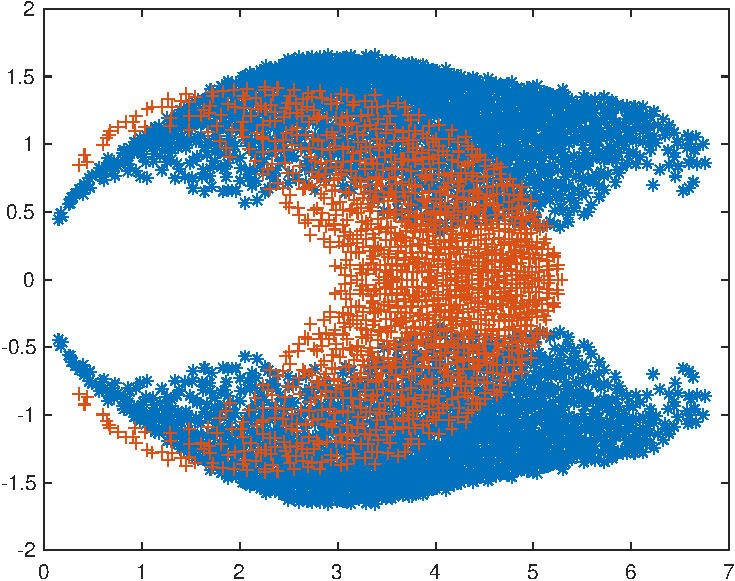
\includegraphics[width=0.325\textwidth]{oddeven_spectrum.pdf}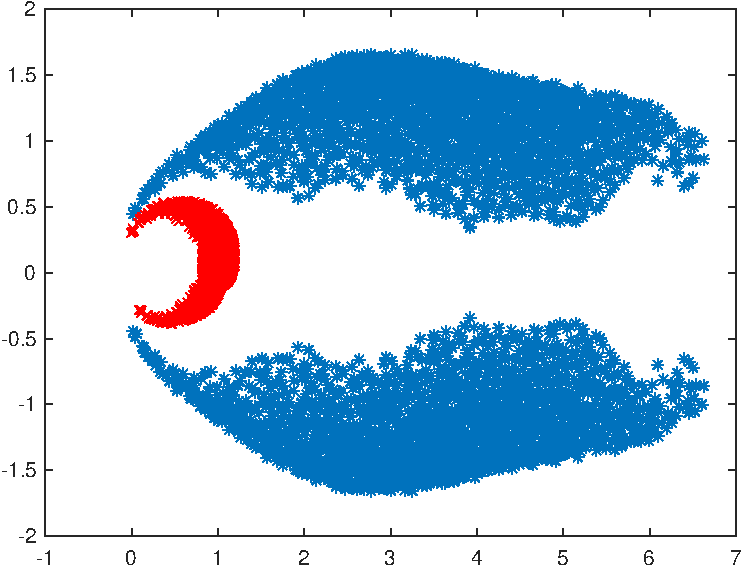
\includegraphics[width=0.335\textwidth]{odd_even_with_Richardson.pdf}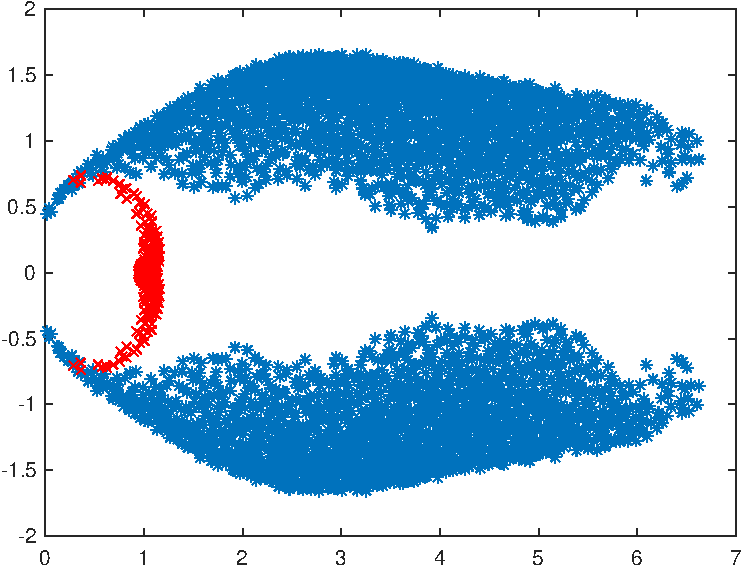
\includegraphics[width=0.335\textwidth]{non_odd_even_with_Richardson.pdf}
\caption{   $4^4$    格子。光谱。左:完整    $D$    的光谱和    $D_{S}$    的光谱(舒尔补)。中:完整    $D$    和    $D p_{R,3}(D)$    的光谱,其中    $p_{R,3}(D)$    为三次理查森多项式。右:完整    $D$    的光谱和    $D M_{3}$    的光谱,其中    $M_{3}$    是通过舒尔补对    $D^{-1}$    进行因式分解,舒尔补的逆    $D_{S}^{-1}$    被    $p_{R,3}(D_{S})$    取代。  } \label{fig:oddeven_spectra_with_Richardson}
\end{figure*}     

DD-   $\alpha$    AMG中奇偶预处理与平滑器的结合方式有两种,第一种方式GMRES、GCR、Richardson均采用这种方式,第二种方式为SAP所特有。  

当将奇偶预处理与 GMRES、GCR 或 Richardson 结合使用时,整个格将以奇偶方式重新排序,然后将所选的迭代方法应用于涉及 Schur 补的求解。另一方面,当与 SAP 结合使用时,重新排序的不是整个格,而是每个域分解块,参见算法 \     \ref{alg:sap}    ,然后使用最小残差求解具有每个块的 Schur 补的线性系统。更具体地说,在算法 \     \ref{alg:sap}    的第 5 行和第 9 行中将奇偶预处理应用于块线性系统。  

对于 SAP 而言,很明显奇偶预处理不会改变其平滑性质,因为它仅帮助 SAP 中的块求解更快地收敛,但此时的问题是它是否有助于 GMRES、GCR 和 Richardson 成为更好的平滑器。我们通过图 \     \ref{fig:oddeven_spectra_with_Richardson}    中中间和右侧面板中显示的光谱来回答这个问题。为此,我们首先声明可以将 Richardson 多项式(即 \  ,   $x^{(k)} = x^{0} + p_{R,k}(D) r^{(0)}$    中的 Richardson 经过    $k$    次迭代后的多项式)写为    $p_{R,k}(D) = ( I-(I-\omega D)^{k} )D^{-1}$    。然后,在中间面板中,我们以红色显示    $\mathrm{spec}\left(Dp_{R,3}(D)\right)$    ,即 \  收缩的光谱。最后,在右侧面板中,我们绘制    $\mathrm{spec}\left(DM_{3}\right)$    ,其中    $M_{3}$    是公式中因式分解形式的    $D^{-1}$    。 \     \ref{eq:Dinv_in_factorized_form}    中的    $D_{S}^{-1}$    被    $p_{R,3}(D_{S})$    取代。显然,在整个晶格上使用奇偶预处理平滑器以及使用 GMRES、GCR 或 Richardson 等迭代方法作用于具有 Schur 补的内部线性系统是有益的,因为右侧面板中的频谱显示出更好地映射到 1.0,以及频谱与零的距离和低模式的散射。  

   \subsection{   \texttt{CUDA}    和    \texttt{HIP}     }     

   \texttt{CUDA}       \cite{NVIDIACU33:online}   (计算统一设备架构)和    \texttt{HIP}       \cite{HIPdocum88:online,HIP_GitHub}   (异构计算可移植接口)是并行计算平台,允许开发人员利用 GPU 的强大功能来加速其应用程序。   \texttt{CUDA}    和    \texttt{HIP}    都提供单指令多线程 (SIMT) 并行编程模型,并提供类似的机制来管理 GPU 上的内存,包括分配、CPU 和 GPU 之间的数据移动以及同步。它们还拥有丰富的基础库,例如线性代数、图像处理和深度学习,以及广泛的开发者社区和生态系统。  

   \texttt{CUDA}    由 NVIDIA 开发,专用于 NVIDIA GPU,使用 NVIDIA 专有的    \texttt{CUDA}    C/C++ 编程语言,而    \texttt{HIP}    则是 AMD 开发的开源替代方案。   \texttt{HIP}    旨在实现跨不同 GPU 架构的可移植性,包括 AMD 和 NVIDIA GPU,支持 C/C++,从而更容易将    \texttt{CUDA}    应用程序移植到    \texttt{HIP}   。  

   \texttt{CUDA}    自 2006 年就已存在,这让它具有了显著的领先优势。它拥有庞大的生态系统,包括成熟的库、工具和广泛的社区支持。然而,   \texttt{CUDA}    将应用程序与 NVIDIA GPU 紧密绑定,限制了它们在不同 GPU 架构之间的可移植性。因此,可以理解的是,针对    \texttt{CUDA}    优化的 NVIDIA GPU 通常可以为某些工作负载提供更好的性能,特别是在深度学习和科学计算等领域。  

   \texttt{HIP}    最显著的优势之一是其跨平台可移植性目标。它使开发人员能够编写可以在不同 GPU 架构上编译和执行的代码,从而使应用程序可以轻松地在 AMD 和 NVIDIA 平台之间转移。在开源策略的鼓励下,HIP 受益于社区贡献、更快的错误修复和其他 GPU 供应商的广泛采用。与    \texttt{CUDA}    的供应商锁定策略相比,   \texttt{HIP}    对 NVIDIA GPU 的支持不如    \texttt{CUDA}    全面。  

总体而言,当针对具有成熟生态系统的 NVIDIA GPU 时,   \texttt{CUDA}    是首选,而    \texttt{HIP}    则在不同 GPU 架构之间提供了更大的灵活性和可移植性。选择取决于项目的具体要求、目标硬件和开发偏好。在这项工作中,我们采用在    \texttt{CUDA}    中开发的代码并将其转换为在 ORISE 超级计算机上使用    \texttt{HIP}    进行编译和运行。  

   \section{数值实验  }       \label{sect:num_exps}     

我们通过比较第    \ref{sect:amg_and_orise}    节中描述的四种迭代方法作为 DD-   $\alpha$    AMG 中的平滑器以及它们与奇偶预处理的相互作用来开始我们的数值实验。我们首先在小节 \     \ref{subsect:smoothers_comp_cpu_only}    中仅在 CPU 上进行此操作。我们已与    \texttt{CUDA}    一起移植并翻译成    \texttt{HIP}    的 DD-   $\alpha$    AMG 代码然后在 ORISE 上运行,并在小节    \ref{subsect:ddalphaamg_on_orise_results}    中展示此结果。最后,我们在小节    \ref{subsect:avx2_on_coarser_levels_results}    中展示通过 AVX 矢量化加速某些粗级内核的结果。在报告求解线性系统的时间时,我们仅报告求解阶段的时间;给出多重网格求解器的设置阶段的时间也意味着对设置阶段的全面讨论,这超出了本文的范围。  

在大多数数值实验中,我们使用的配置的详细信息列在表    \ref{tab:config}    中。此时,重要的是要注意此配置需要多重网格。它的介子质量为 135 MeV,与其物理值相对应,这将导致相当病态的线性系统。为了举例说明,我们使用 DD-    $\alpha$    AMG 解决了此配置的线性系统,同时使用 BiCGStab 和三级多重网格作为 FGMRES    \cite{rottmann2016adaptive}    的预处理器,具有奇异和轻夸克质量。两级多重网格方法的参数可以在表 \     \ref{tab:parameter}    中找到。此次运行是在 9 个 ORISE 节点上使用仅 CPU 代码完成的,相对残差容差为    $10^{-10}$   。对于奇异夸克质量,使用 BiCGStab 需要 23.9 秒,而使用多重网格则需要 11.3 秒。当我们切换到轻夸克质量时,时间分别变为 590.2 秒和 31.5 秒。这些时间说明了如果没有多重网格,模拟可能会变得不可行,因为总体执行时间通常由此处研究的线性系统的解决定。  

   \subsection{平滑器:仅 CPU 比较  }       \label{subsect:smoothers_comp_cpu_only}     

我们首先通过实现带有和不带有奇偶预处理的 CPU 版本的 GCR 和 Richardson 来扩展 DD-   $\alpha$    AMG 的功能。在此之前,DD-   $\alpha$    AMG 只能使用 SAP 或 GMRES 作为平滑器运行。现在我们对这四种平滑器进行比较,以评估它们的有效性和实践中的差异。为了进行这种比较,我们在类似条件下(例如初始随机种子、并行化、Arnoldi 过程的重启长度等)使用所有这些平滑器运行了两级多重网格方法。这些运行的结果可以在表 \     \ref{tab:smoothers_cpu_only_comparison}    中找到,两级方法的参数可以在表 \     \ref{tab:parameter}    中找到。  

为了比较不同平滑器的优缺点,我们测试了有或没有奇偶预处理和奇异或轻夸克质量的四种组合。从表 \     \ref{tab:smoothers_cpu_only_comparison}    中我们可以看出,如果没有奇偶预处理,SAP 就是最有效的平滑器,无论是在收敛性方面还是在多重网格求解器的执行时间方面,部分原因是它最有效地抑制了误差的高频分量。此外,由于我们只在 SAP 中进行局部求解,因此与 GMRES 和 GCR 相比,缓存非常有利,从而导致前者迭代方法每次迭代所需的时间更短。将 GMRES 与 GCR 进行比较时,后者每次迭代所需的时间更长,这与    \cite{elman1982iterative}    和小节 \     \ref{subsubsect:gcr}    中的讨论相符。总体而言,在没有奇偶预条件的情况下,理查森方法不够有竞争力,因为它导致整个多重网格方法在奇异夸克质量情况下的收敛性非常低,而在轻夸克质量情况下则根本不收敛。  

与其他三种平滑器相比,当我们打开奇偶预处理时,Richardson 的情况发生了很大变化。在这种情况下,对于两种夸克质量值,Richardson 的多重网格求解速度几乎与 SAP 和 GMRES 一样快;与 SAP 相比,差异仅为 10 \%。奇偶 Richardson 与其他三种平滑器相比有两个明显优势:除了在迭代次数和多重网格求解器的执行时间方面具有竞争力的平滑器效率外,它的内存要求极低,并且是迄今为止这些方法中最简单的实现方法,这些特性在试图实现可移植性和简单性但同时又快速且内存消耗低的代码中非常具有吸引力。  

我们注意到,尽管我们在 \     \ref{tab:smoothers_cpu_only_comparison}    表中的一些不同情况下使用了 Richardson 的    $\delta$    的不同值,但    $\delta=1.5$    的值在给出近似最佳收敛方面似乎足够通用。  

我们现在在 GPU 上探索这些平滑器。由于与上面考虑的其他三种平滑器相比,GCR 所需的时间和内存更大,因此我们将此方法排除在下一节的讨论之外。  

   \begin{table*}[h]
    \centering
    \caption{使用仅 CPU 代码对 DD-   $\alpha$    AMG 中不同平滑器(即 SAP、GMRES、GCR 和 Richardson 迭代)的比较时间,适用于奇异和轻夸克质量。在所有情况下都使用了两级方法。所有运行都在 ORISE 中的 4 个节点上完成。时间以秒为单位。通过破折号我们表明该方法没有收敛。  }
   \label{tab:smoothers_cpu_only_comparison}
   \begin{tabular}{ccccccc}
     \hline
      & mass                     & smoother       & FGMRES iters & smoothing time & coarse time & solve time   \\  \hline
      &                          & SAP(3,4)       & 22           & 169.83         & 34.33       & 245.27       \\ 
      & \multirow{2}{*}{        $m_{s}$        } & GMRES(3,4)     & 24           & 278.12         & 37.88       & 364.21       \\ 
      &                          & GCR(3,4)       & 24           & 354.89         & 36.75       & 437.86       \\ 
      &                          & Richardson(12,1.7) & 95          & 750.03         & 92.08        & 1028.93       \\ 
     non odd-even &&&&&& \\ [-1.5ex]
     \cline{2-7}
     &&&&&& \\ [-1.5ex]
      &                          & SAP(3,4)       & 43   & 337.35 & 693.92 & 1122.45  \\ 
      & \multirow{2}{*}{        $m_{l}$        } & GMRES(3,4)     & 55   & 639.47 & 939.22 & 1693.01  \\ 
      &                          & GCR(3,4)       & 53   & 797.05 & 893.82 & 1812.04  \\ 
      &                          & Richardson(12,1.5) & -    & -      & -      & -        \\ 
          &&&&&& \\ [-1.5ex]
          \hline
          &&&&&& \\ [-1.5ex]
          &                           & SAP(3,4)       & 16  & 70.3   & 6.73  & 96.94   \\ 
          &  \multirow{2}{*}{        $m_{s}$        } & GMRES(3,4)     & 13  & 73.56  & 6.23  & 96.70   \\ 
          &                           & GCR(3,4)       & 13  & 92.15  & 6.08  & 115.51  \\           
          &         & Richardson(12,1.5) & 15   & 72.02  & 7.45 & 100.46       \\   
     odd-even     &&&&&& \\ [-1.5ex]
     \cline{2-7}
          &&&&&& \\ [-1.5ex]
          &         & SAP(3,4)        & 23  & 100.58  & 166.72  & 300.26   \\ 
          & \multirow{2}{*}{        $m_{l}$        }         & GMRES(3,4)      & 23  & 131.63  & 145.27  & 310.19   \\ 
          &    
          & GCR(3,4)         & 23  & 171.27   & 153.03   & 366.15    \\           
          &         & Richardson(12,1.5) & 28   & 135.05  & 163.21 & 335.84       \\   
          \hline
   \end{tabular}
   \end{table*}     

   \subsection{DD-    $\alpha$    AMG 通过 ORISE 上的    \texttt{HIP}     }       \label{subsect:ddalphaamg_on_orise_results}     

在此工作之前,通过    \texttt{CUDA}    移植的 DD-    $\alpha$    AMG 中的唯一函数是双精度最精细级 SAP 和最精细级 Dirac 运算符。我们通过移植奇偶预处理版本的 GMRES 和 Richardson(也通过    \texttt{CUDA}    )扩展了此功能。为此,我们利用了一些现有的    \texttt{CUDA}    内核(之前在移植最精细级 SAP 和双精度 Dirac 运算符时开发),并创建了一些我们自己的内核,以便首先获得能够在 GPU 上运行的 Schur 补(参见方程 \     \ref{eq:schur_complement}   )。以 GPU 版本的 Schur 补为基础,奇偶 GMRES 和 Richardson 均围绕它构建,而 GMRES 显然需要更多的开发时间,因为它需要内积、最小二乘最小化等。  

同样,与 CPU 的情况一样,我们在类似条件下比较了 SAP、GMRES 和 Richardson,其结果显示在表 \     \ref{tab:comp-cpu-gpu}    中。  

由于已经在 \     \ref{tab:smoothers_cpu_only_comparison}    表中彻底比较了多重网格环境中的不同平滑器,因此我们现在在 \     \ref{tab:comp-cpu-gpu}    表中仅关注平滑器所花费的时间;这些时间来自对多个多重网格求解的平均平滑时间。我们在 \     \ref{tab:comp-cpu-gpu}    表中显示了最佳 CPU 时间与最佳 GPU 时间。SAP 的优势不仅在 CPU 上很明显,而且在 GPU 上也很明显,前者是由于 CPU 缓存使用率高,后者是由于 SAP 块的独立性,从而可以在 GPU 上异步启动所有这些独立块的操作。SAP 相对于 GMRES 的另一个优势是,点积在格上具有局部性而非全局性。  

尽管奇偶 Richardson 主要由全局 Schur 补码的应用组成,但 \     \ref{tab:comp-cpu-gpu}    表显示,此迭代方法一次调用的平均时间与 GPU 上的 SAP 大致相同。这使得 Richardson 在被视为 GPU 上的多重网格平滑器时再次具有竞争力,并且当实现简单性和低内存消耗至关重要时,这将再次成为平滑器的首选。  

   \begin{table}
    \centering
    \caption{比较 GPU 和 CPU 上不同平滑器的性能。运行于 4 个节点,每个节点有 4 个 MPI 进程,每个进程有 1 个 GPU 和 4 个 OpenMP 线程。时间以秒为单位,对应于一次平滑器调用的平均时间。  }
    \label{tab:comp-cpu-gpu}
    \begin{tabular}{cccc}
    \hline
    smoother   & CPU     & GPU     & speedup    \\  \hline
    SAP(3,4)   & 4.39    & 0.33    & 13.30       \\ 
    GMRES(3,4) & 5.66    & 0.45    & 12.60      \\ 
    Richardson & 4.80    & 0.36    & 13.33      \\  \hline
    \end{tabular}
\end{table}     

   \subsection{CPU 改进  }       \label{subsect:avx2_on_coarser_levels_results}     

在 DD-    $\alpha$    AMG    \cite{wuppertalGPUDDalphaAMG}    的混合 CPU+GPU 实现中,最精细平滑器和最精细狄拉克算子在 GPU 上运行,求解器可能通过粗网格计算得到进一步改进。自其原始版本    \cite{wuppertalDDalphaAMG}    以来,DD-    $\alpha$    AMG 中使用    \texttt{SSE}    进行矢量化,以加速执行最苛刻的操作,例如在不同级别应用狄拉克算子时的 \ 。我们扩展了一些矢量化粗网格内核,以支持    \texttt{AVX2}    和    \texttt{AVX-512}   。  

在    $l$    级别,对于    $l>1$    ,两个相邻站点之间的交互被编码为    $2N_{v} \times 2N_{v}$    密集复数矩阵,其中    $N_{v}$    是在级别    $l-1$    选择的测试向量的数量。这些小而密集的矩阵向量乘积中隐含的数据结构和操作与使用    \texttt{SSE}    等矢量化方案具有自然兼容性。由于缓存行大小通常为 64 B,因此相应的 16 个单精度数字与    \texttt{SSE}    、    \texttt{AVX2}    和    \texttt{AVX-512}    中的寄存器自然匹配,其中矢量化寄存器的大小分别为 4、8 和 16,此外    $2N_{v}$    的值通常是这些矢量化寄存器大小的倍数。  

尽管所有这些数据大小都很好地匹配,但在应用狄拉克算子    $D_{l}$   、   $l>1$    时,需要遍历这些小而密集的矩阵向量乘积序列,而不会将一个矩阵向量乘法的数据重用到下一个矩阵向量乘法中。因此,在单次应用狄拉克算子时,执行时间受到内存带宽的高度限制。在仅应用一次    $D_{l}$    的情况下,从    \texttt{SSE}    升级到    \texttt{AVX2}    或    \texttt{AVX-512}    可能没有什么好处。但如果多次应用    $D_{l}$   ,我们是否能从    \texttt{AVX}    中受益将取决于    $D_{l}$    所需的数据以及这与缓存大小的比较情况。  

如果我们取    $N_{v}=24$    ,那么    $D_{l}$    (    $l>1$    ) 内的其中一个小密集矩阵将以单精度占用    $48 \times 48 \times 2 \times 4 = 18.0$    KB 的数据。例如,Intel(R) Xeon(R) Platinum 8180 节点每个核心具有 32 KB 的 L1 缓存,这只允许托管其中一个小密集矩阵,但另一方面,它的 L3 缓存为 38.5 MB,最多可容纳 2,190 个这样的矩阵。Dirac 运算符需要每个块行存储大约九个    $2N_{v} \times 2N_{v}$    块。由于每个块行直接映射到单个格点,因此我们可以在 L3 缓存中放置的最大点数大约为 243。运行 GMRES 等迭代方法时,请参阅 alg。 \     \ref{alg:gmres}    ,狄拉克算子每次迭代应用一次,因此如果迭代方法需要多次迭代,并且该方法所需的所有数据都适合缓存,那么从    \texttt{SSE}    升级到    \texttt{AVX}    会带来好处。GMRES 等方法所需的数据将是狄拉克算子加上多个向量的数据,例如 \  Arnoldi 向量和一些缓冲区。我们现在通过 DD-    $\alpha$    AMG 和我们通过    \texttt{AVX}    包含在其中的矢量化升级来验证这些考虑因素。  

在与之前相同的 Xeon 节点上,我们针对底层晶格大小为    $8^4$    的规范配置运行 DD-    $\alpha$    AMG 的两级方法。我们对两种聚合大小    $2^4$    和    $4^4$    执行此操作,分别得到    $4^4$    和    $2^4$    的粗网格。   $4^4$    的粗网格共有 256 个晶格点,如上所述,无法放入 L3 缓存中。另一方面,   $2^4$    的粗网格共有 16 个点,其狄拉克算子所需的全部数据可放入 L3 中。我们建立了一个测试,其中我们总共调用粗网格狄拉克算子 10,000 次。我们多次运行此实验,对结果执行时间取平均值,并将结果显示在 tab.s \     \ref{tab:avx_vs_sse_coarse_grid_Dirac_4to4}    和    \ref{tab:avx_vs_sse_coarse_grid_Dirac_2to4}    中。来自 Dirac 算子应用中的光环交换的通信开销不允许我们看到矢量化升级的裸露影响。因此,我们还使用修改后的 Dirac 算子运行了测试,其中我们禁用了那些最近邻数据传输,我们还分别在 tab.s    \ref{tab:avx_vs_sse_coarse_grid_Dirac_4to4}    和    \ref{tab:avx_vs_sse_coarse_grid_Dirac_2to4}    中包括了针对    $4^4$    和    $2^4$    粗网格的传输时间。  

   \begin{table}
    \centering
    \caption{对于对应于    $4^4$    晶格的粗网格狄拉克算子,   \texttt{AVX2}    和    \texttt{AVX-512}    与    \texttt{SSE}    相比的时间和加速比。所有时间均以秒为单位,对应于以单精度应用粗网格狄拉克算子共 10,000 次所需的平均时间。   \texttt{AVX2}    和    \texttt{AVX-512}    括号中的数字是相对于    \texttt{SSE}    情况的加速比。第一列表示我们是否已关闭狄拉克算子中的光晕交换。  }
    \label{tab:avx_vs_sse_coarse_grid_Dirac_4to4}
    \begin{tabular}{ccccc}
    \hline
    comm.s                 &  \#  MPI   & SSE   & AVX2        & AVX-512      \\ 
                           & Proc.s   &       &             &              \\  \hline
    \multirow{5}{*}{ON}    & 2        & 13.9  & 9.7  (1.43) & 9.5 (1.46)   \\ 
                           & 4        & 7.64  & 5.39 (1.42) & 5.3 (1.44)   \\ 
                           & 8        & 4.5   & 3.47 (1.3)  & 3.2 (1.41)   \\ 
                           & 16       & 2.4   & 2.01 (1.19) & 1.89 (1.27)  \\ 
                           & 32       & 2.33  & 1.96 (1.19) & 1.91 (1.22)  \\  \hline
    \multirow{5}{*}{OFF}   & 2        & 12.9  & 9.2 (1.4)   & 9.02 (1.43)  \\ 
                           & 4        & 7.0   & 4.9 (1.43)  & 4.64 (1.5)   \\ 
                           & 8        & 3.7   & 2.4 (1.54)  & 2.37 (1.56)  \\ 
                           & 16       & 2.1   & 1.6 (1.3)   & 1.53 (1.37)  \\ 
                           & 32       & 1.3   & 1.03 (1.26) & 0.97 (1.34)             \\  \hline
    \end{tabular}
\end{table}     

   \begin{table}
    \centering
    \caption{对于对应于    $2^4$    晶格的粗网格狄拉克算子,   \texttt{AVX2}    和    \texttt{AVX-512}    与    \texttt{SSE}    相比的时间和加速比。所有时间均以秒为单位,对应于以单精度应用粗网格狄拉克算子共 10,000 次所需的平均时间。   \texttt{AVX2}    和    \texttt{AVX-512}    括号中的数字是相对于    \texttt{SSE}    情况的加速比。第一列表示我们是否已关闭狄拉克算子中的光晕交换。  }
    \label{tab:avx_vs_sse_coarse_grid_Dirac_2to4}
    \begin{tabular}{ccccc}
    \hline
    comm.s                 &  \#  MPI   & SSE   & AVX2        & AVX-512      \\ 
                           & Proc.s   &       &             &              \\  \hline
                           & 2        & 0.97  & 0.67 (1.45) & 0.62 (1.56)  \\ 
    \multirow{2}{*}{ON}    & 4        & 0.62  & 0.42 (1.48) & 0.31 (2.0)   \\ 
                           & 8        & 0.4   & 0.28 (1.43) & 0.24 (1.67)  \\  \hline
                           & 2        & 0.86  & 0.56 (1.54) & 0.48 (1.8)   \\ 
    \multirow{2}{*}{OFF}   & 4        & 0.47  & 0.26 (1.8)  & 0.19 (2.47)  \\ 
                           & 8        & 0.26  & 0.16 (1.6)  & 0.11 (2.36)  \\  \hline
    \end{tabular}
\end{table}     

正如预期的那样,从    \texttt{AVX}    到    \texttt{SSE}    的时间减少在 \     \ref{tab:avx_vs_sse_coarse_grid_Dirac_2to4}    表中比在 \     \ref{tab:avx_vs_sse_coarse_grid_Dirac_4to4}    表中更大。这仅仅是因为在后一种情况下缓存未命中次数更多,其中    $D_{l}$    所需的全部数据无法完全存储在 L3 中。值得注意的是,与    \texttt{AVX2}    相比,   \texttt{AVX-512}    通常以较低的频率运行,因此前者实现的加速远非后者的两倍,这与我们在 \     \ref{tab:avx_vs_sse_coarse_grid_Dirac_2to4}    表中的结果一致。  

最后,当我们使用    \texttt{SSE}   (   $4^4$    和四个 MPI 进程的集合)针对同一    $8^4$    问题运行整个 DD-    $\alpha$    AMG 求解器时,粗网格总共需要 0.0825 秒的时间,而使用    \texttt{AVX2}    和    \texttt{AVX-512}    分别需要 0.0616 和 0.0517 秒。GMRES 中的    \texttt{AVX}    未升级的多个开销和区域是未看到表 \     \ref{tab:avx_vs_sse_coarse_grid_Dirac_2to4}    中建议的 1.48 和 2.0 加速的原因。这促使我们在 GMRES    \cite{loe2022toward}    中对狄拉克算子使用多项式预处理,正如在    \cite{espinoza2023coarsest}    中实现和分析的那样。此外,关闭通信时,表    \ref{tab:avx_vs_sse_coarse_grid_Dirac_4to4}    和    \ref{tab:avx_vs_sse_coarse_grid_Dirac_2to4}    中获得的卓越加速表明,使用避免通信的 Krylov 方法    \cite{hoemmen2010communication}    会带来益处。  

我们从    \ref{tab:avx_vs_sse_coarse_grid_Dirac_4to4}    和    \ref{tab:avx_vs_sse_coarse_grid_Dirac_2to4}    表中注意到,由于我们在不同的运行中更改并行性,矢量化导致的加速不一致。获得更好、更统一(即 \  并行性独立)矢量化性能的一种可能方法是扩展求解器以支持多个右侧    \cite{yamamoto2022implementation}    ;当将 Dirac 运算符应用于多个向量时,必须将每个    $2N_{v} \times 2N_{v}$    块应用于多个向量,这可以成为高度缓存友好的操作。  

最后,我们注意到,使用    \texttt{AVX}    对 ORISE 的益处不大,我们的数值测试显示,与    \texttt{SSE}    实现相比,其速度最多提升 1.1 倍。我们认为这是因为从该机器的主内存中获取数据所花费的时间特别长。  

   \section{结论和未来工作  }       \label{sect:conclusions_and_future_work}     

我们扩展了 DD-    $\alpha$    AMG 求解器的 CPU 专用版本,以允许使用两个新的平滑器,即 GCR 和 Richardson。在此过程中,我们已经表明,由于时间和内存的原因,GCR 不是一个好的选择。另一方面,Richardson 因其实现简单、内存要求低和具有竞争力的效果而成为一种非常有吸引力的替代方案。此外,从通过    \texttt{CUDA}    移植 SAP 的现有 DD-    $\alpha$    AMG 的 CPU+GPU 版本,我们移植了 GMRES 和 Richardson,这不仅增强了 SAP 作为平滑器在 CPU 上的优势,也增强了 SAP 作为平滑器在 GPU 上的优势,同时在某些方面重申了 Richardson 作为 CPU 和异构架构上多重网格平滑器的潜在和可能的优势。最后,通过    \texttt{AVX2}    和    \texttt{AVX-512}    ,粗网格昂贵的 CPU 内核变得更快。本文对 DD-   $\alpha$    AMG 的这些改进带来的好处进行了彻底的分析。  

即将开展的工作源自上述改进和扩展。例如,在其他 LQCD 多重网格求解器中使用 Richardson 作为平滑器就是其中一种途径。另一个可能的工作方向是在 DD-   $\alpha$    AMG 中较粗的级别上使用较低精度(例如 \  half)与高级矢量化(例如    \texttt{AVX-512}   )相结合。  

   \section{致谢  }    我们非常感谢杨一博为我们提供规范配置。Gustavo Ramirez-Hidalgo 的工作得到了德国研究基金会 (DFG) 研究部门 FOR5269“研究 QCD 中受限胶子的未来方法”的支持。  

   \appendix     

   \section{配置和求解器参数  }     

我们使用的仪表配置列于表~    \ref{tab:config}    中。DD-    $\alpha$    AMG 中使用的参数列于表~    \ref{tab:parameter}    中。  

   \begin{table}[H]
        \centering
        \caption{配置与其参数一起使用。由 C11P14L    \cite{LIU2023137941}    提供。  }\label{tab:config}
        \begin{tabular}{cc}
        \hline
        Lattice size (        $N_t \times N_s^3$        )    &         $96\times 48^3$           \\ 
        Pion mass (        $m_{\pi}$        )                & 135               \\ 
        Clover term (        $c_{sw}$        )               & 1.16058719        \\ 
        light mass (        $m_{l}$        )                 & -0.2825           \\ 
        strange mass (        $m_{s}$        )               & -0.2310           \\  \hline
        \end{tabular}
\end{table}     

   \begin{table}[H]
    \centering
    \caption{以 SAP 为平滑器的两级 DD-    $\alpha$    AMG 的默认参数。这些是使用轻夸克质量    $m_{l}$    求解时使用的值。对于奇异夸克质量,   \texttt{number of setup iterations}    的值变为 3。  }
    \label{tab:parameter}
    \begin{tabular}{ccc}
    \hline
    parameter                          &         $l=1$              &         $l=2$               \\ \hline
    number of setup iterations         &   5        & -           \\ 
    number of test vectors             &   20       & -           \\ 
    aggregate size                     &         $4^4$              & -           \\ 
    restart length of (F)GMRES         & 10         & 200          \\ 
    maximum restarts of (F)GMRES       & 10         & 10          \\ 
    (F)GMRES rel. \  residual tolerance  &         $10^{-10}$         &         $10^{-1}$           \\ 
    post-smoothing steps               & 3          & -           \\ 
    Minimal Residual iterations        & 4          & -           \\ \hline
    \end{tabular}
\end{table}     

   \bibliographystyle{model1-num-names}    
   \bibliography{cas-refs}     


  
\end{document}

